\chapter{Design}
In this section, we will describe the internal details of the components in the architecture specifically on how the scheduling algorithms work in order to realize the negotiation, the meaning of job mappings, resource offers and feedback reports. 
\label{chapter:ischeduler}
\section{Entities}
A design entity is an element(component) of a design that is structurally and functionally distinct from other elements and that is separately named and referenced. They result from the decomposition of the software system requirements. The objective is to divide the system into separate components that can be considered, implemented, changed, and tested with minimal effect on other entities. Examples of design entities are: \textbf{\textit{protocol, application layer, state machine, data model, object, task, sub-systems, modules}} etc.\\ \\
\textbf{Job Mappings}\\
A job mapping is basically a job and its allocated set of resources. A forward job record is a job mapping and other related job details important for its launch. A list of such forward job records are sent by the batch scheduler in response to receiving a resource offer from the runtime scheduler.\\
%\vspace{-0.5in}
%\begin{center}
\begin{equation*}
%\begin{multlined}
\begin{aligned}
&M_{i}\ \ \ \textit{:=\ \ \ Job Mapping\ \ \ :=}\ \ \ \{jobid,node count,bitmap\}\\
&Map_{i}\ \ \ \textit{:=\ \ \ Forward Job Record\ \ \ :=}\ \ \ \{M_{i},details_{i}\}\\
&Map\ \ \ \textit{:=\ \ \ {$<Map_{1}><Map_{2}>...<Map_{n}>$}}
%\end{multlined}
\end{aligned}
\end{equation*}
%\end{center}
In the above description $details_{i}$ refers to the details of any $i^{th}$ job such as \textit{constraints, priority, runtime estimate, max nodes, min nodes, job name, start time, deadline}. In these details, the constraints are specific to the purpose of negotiation and this can be related to node count that the job is requesting for, memory size, exclusive / shared resource access etc. Currently, we support only the constraints for node count. The node count constraint will again have a min and max both of which will fall within the window of max and min nodes of the job. It is using these constraints that the batch scheduler will negotiate with the runtime scheduler and with every negotiation attempt it will relax the constraints to bargain better.\\ \\
\textbf{Resource Offers}\\
A reservation is basically a job being guaranteed a set of resources for a certain period of time. A resource offer is a list of such reservations and the set of nodes which are free in the partition after the runtime scheduler has guaranteed these reservations. The runtime scheduler will send such a resource offer to the batch scheduler if it rejected its mapping or it is sending a new offer that it generated.\\
%\vspace{-0.5in}
%\begin{center}
\begin{equation*}
%\begin{multlined}
\begin{aligned}
&Resv_{i}\ \ \ \textit{:=\ \ \ Job Reservation\ \ \ :=}\ \ \ \{jobid,node count,bitmap,start time,end time\}\\
&IdleNodes\ \ \ \textit{:=\ \ \ Residual Nodes\ \ \ :=}\ \ \ \{bitmap\}\\
&Offer\ \ \ \textit{:=\ \ \ $<Resv_{1}><Resv_{2}>...<Resv_{n}>$,\ IdleNodes}
%\end{multlined}
\end{aligned}
\end{equation*}
%\end{center}
The \textbf{\textit{$Resv_{i}$}} entry in the resource offer corresponding to a particular job id must match the job id of the \textbf{\textit{$Map_{i}$}} entry in the forwarded jobs. This means that the sequence in which jobs were forwarded to runtime scheduler will be the same sequence of jobs for which reservations will be sent to the batch scheduler.\\ \\
%%%%%%%%%
\textbf{Feedback Reports}\\
Periodic or event-driven feedback reports on the latest status of the running jobs are sent by the runtime scheduler to the batch scheduler. It is event-driven for events such as job termination, job completion, acceptance of a mapping received from batch scheduler.
%\vspace{-0.2in}
%\begin{center}
\begin{equation*}
%\begin{multlined}
\begin{aligned}
&P_{i}\ \ \ \textit{:=\ \ \ Performance Data\ \ \ :=}\ \ \ \{model,energy,io,memory,hint\}\\
&Report_{i}\ \ \ \textit{:=\ \ \ Status Report\ \ \ :=}\ \ \ \{jobid,node count,bitmap,run time,end time,state,P_{i}\}\\
&Feedback\ \ \ \textit{:=\ \ \ $<Report_{1}><Report_{2}>...<Report_{n}>$}
%\end{multlined}
\end{aligned}
\end{equation*}
The feedback reports can also contain performance specific data such as energy consumption, performance model of completed jobs that can be used by batch scheduler for making better decisions on same jobs submitted again in the future. For running jobs, the reports can contain similar information but most important ones would be the current assigned node count, expected end time, memory usage etc.
%\end{center}
%%%%%%%%%%
\section{Scheduling Algorithms}
<Include the decision logic algorithm also here in this section>
Following pages present the pseudo code for both the batch and runtime scheduling algorithms. 
\subsection{Batch Scheduling}
%\clearpage
%%%%%%
%%%%%%
%\RestyleAlgo{boxed}
\RestyleAlgo{boxruled}
\IncMargin{1em}
\begin{algorithm}[!htbp]
 \DontPrintSemicolon
 \KwData{Resource Offer}
 \KwResult{Map : Jobs $\rightarrow$ Offer}
 build invasive job queue\;
 \If{empty queue}{
  return empty Map\;
 }
 sort queue by job priorities\;
 reservations $\leftarrow$ Offer.Reservations\;
 freenodes $\leftarrow$ Offer.ResidualNodes\;
 \While{not at end of the invasive job queue}{
  read queue entry\;
  \If{entry.jobId in reservations}{
   resv $\leftarrow$ reservations(entry.jobId)\;
   \eIf{resv.bitmap is NULL}{
    entry.start\_time $\leftarrow$ resv.start\_time\;
    entry.node\_count $\leftarrow$ $0$\;
    adjustNodeCount(entry.jobId)\;
   }{
    entry.start\_time $\leftarrow$ $0$\;
    entry.node\_count $\leftarrow$ resv.node\_count\;
    entry.bitmap $\leftarrow$ resv.bitmap\;
    create forward job record using entry\;
    append record to Map\;
    mapped $\leftarrow$ true\;
   }
  }
  \If{mapped is true}{
   continue\;
  }
  try mapping to the residual nodes\;
  \If{successfully mapped}{
   update the residual nodes\;
  }
  create forward job record using entry\;
  append record to Map\; 
 }
 try\_to\_best\_fit(Map, invasive job queue, Offer)\;
 return Map\;
 \caption{Batch Scheduling Algorithm}
 \label{algo:1}
\end{algorithm}
%%%%%%%
\textbf{\textit{Algorithm }}\ref{algo:1} presents a high level pseudo code of the batch scheduling algorithm. Following points describe the algorithm:
\begin{itemize}
\item It takes as input a resource offer from iRTSched and maps jobs from its queue to the offered resources.
\item \textbf{\textit{Line \boldmath{$1$}}}: A separate job queue is constructed by scanning the main job queue for jobs which have been submitted specifically to the invasic partition. These jobs are then sorted according to their priorities.
\item \textbf{\textit{Line \boldmath{$8$-$34$}}}: For every job in the invasive queue: If it is found in the reservation list from the resource offer and if it can start immediately(has a bitmap allocated) then we will just append this to the Map after creating a new forward job record.
\item If it starts in future(has a NULL bitmap) then we will relax its node count constraints by a step size calculated as below and try to map it to the residual nodes.
\vspace{-0.30in}
\begin{center}
\boldmath\begin{equation*}
step\ size = \frac{(Job.MaxNodes - Job.MinNodes)}{MAX\_NEGOTIATION\_ATTEMPTS}
\end{equation*}
\end{center}
\item If \textbf{\textit{step size}} in the above calculation comes up as $0$ then we will set it as $1$.
\item \textbf{\textit{job.node\_count.min $=$ job.node\_count.min - step size}}. If the computed value is negative or less than the job's minimum number of nodes then we just set \textbf{\textit{job.node\_count.min $=$ job.min\_nodes}}.
\item If the job is not found in the reservation list then this must be a new job that was submitted after the previous dispatch of jobs was completed by batch scheduler in the previous negotiation attempt. We will directly try to map it to the residual nodes.
\item If a job could not be mapped, then we will just append it to the Map by creating a new forward job record. If it was mapped, then we will set the current node count of that job to the count of the allocated nodes. The node count constraints remain the same.
\item \textbf{\textit{Line \boldmath{$35$}}}: We will try to map batch jobs that could not be mapped due to lack of sufficient resources in the offer by shrinking jobs which have been currently mapped. The shrink operation considers mapped jobs in the reverse order of their priority so that the operation can start from the lowest priority mapped job till the highest one.
\item Result would be a best fit mapping of the invasic jobs ready to be forwarded to iRTSched.
\item \textbf{\textit{Algorithm 2:}} This algorithm shows how the best fit mapping is computed. It considers all those jobs which could not be mapped. For every such job, it will try to shrink the mapped jobs in an increasing order of priorities until sufficient nodes have been found to map the job. 
\item If we were successful in mapping any new jobs by shrink operations, then we must rescan the invasive job queue to fill the Map by jobs which had been previously skipped due to a limit on the reservation depth. This means that we have a limit on the number of jobs that have not been successfully mapped to be forwarded to runtime scheduler.
\item \textbf{\textit{Algorithm 3:}} This algorithm shows how the analysis of running jobs are done in order to shrink them to satisfy a job request. Analysis will consider shrinking the jobs by a step size computed as shown below. If analysis is successful, then jobs are shrunk.
\vspace{-0.30in}
\begin{center}
\boldmath\begin{equation*}
step\ size = \frac{(Job.node\_cnt - Job.node\_count.min)}{MAX\_NEGOTIATION\_ATTEMPTS}
\end{equation*}
\end{center}
\end{itemize}
Batch scheduler will provide \textbf{\textit{fairness}} to jobs while scheduling by considering them in the order of decreasing priorities. It also avoids any \textbf{\textit{job starvation}} by forwarding jobs that could not get mapped to the available resource offer. This will result in the runtime scheduler giving these jobs future start times as per its backfill algorithm and only then process other job requests after it  in the list of forwarded jobs. Batch scheduler will also adjust the expected end times of those jobs that it will transform by expand / shrink. This adjustment will take into consideration the performance model of the running application.
%%%%%%
\setcounter{AlgoLine}{0}
%%%%%%%
%\pagebreak
%\newpage
\begin{algorithm}[!htbp]
 \DontPrintSemicolon
 \KwData{Map, Invasive Job Queue, Offer}
 \KwResult{Updated Map : Jobs $\rightarrow$ Offer}
 avail\_bitmap $\leftarrow$ Offer.ResidualNodes\;
 \While{not at end of the Map}{
  read Map entry\;
  \If{(entry.start\_time EQ $0$) AND (entry.bitmap NEQ NULL)}{
   continue\;
  } 
  \tcc{Try to map this job by shrinking other mapped jobs}
  try\_sched(entry, Map, avail\_bitmap)\;
  \If{successfully scheduled}{
   update avail\_bitmap\;
  }
 }
 \If{avail\_bitmap not empty}{
  Rescan the invasive job queue to fill the residual nodes with some new jobs\;
 }
 \caption{Best Fit Algorithm}
\end{algorithm}
\setcounter{AlgoLine}{0}
%%%%%%%%%
%\IncMargin{1em}
\begin{algorithm}[!htbp]
 \DontPrintSemicolon
 \KwData{Entry, Map, avail\_bitmap}
 \KwResult{Updated entry: Mapped to some nodes}
 \tcc{The mapped jobs in the Map would be analyzed in the reverse order which is increasing in the priority}
 Analyze in increasing order of priority if the mapped jobs in the Map can be shrunk to find enough nodes for entry\;
 \If{sufficient nodes available}{
  shrink the mapped jobs as per the analysis\;
 }
 entry.bitmap $\leftarrow$ bitmap(available nodes)\;
 \caption{Try Schedule Algorithm}
\end{algorithm}
\setcounter{AlgoLine}{0}
%%%%%%%
\subsection{Runtime Scheduling}
\begin{algorithm}[!t]
 \DontPrintSemicolon
 \KwData{Attempts, Jobs2Map, Error Code, Offer<empty>}
 \KwResult{Offer<Reservations, Residual nodes>}
 \If{Error Code is SUCCESS}{
 \tcc{Batch Scheduler accepted the previously sent offer}
  \If{(Jobs2Map NEQ NULL) AND (Attempts GT $1$)}{
   initialize runtime state\;
  }
  \tcc{Repeat the transformation of the system which was done for the previous attempt}
  schedule((Attempts GT $1$) ? (Attempts - 1) : Attempts, Jobs2Map, Error Code, Offer)\;
  \tcc{Offer being generated for the first time if attempts is equal to $1$}
  \If{Attempts EQ $1$}{
   return SUCCESS\;
  }
  \If{schedule was successful AND Jobs2Map NEQ NULL AND Attempts GT $1$}{
   commit the mapped jobs to the running list\;
   return SUCCESS\;
  }
 }
 \tcc{Batch Scheduler rejected the previously sent offer}
 \If{Error Code NEQ SUCCESS}{
  initialize runtime state\;
  schedule(Attempts, Jobs2Map, Error Code, Offer)\;
 }
 return error code\; 
 \caption{Algorithm for generating a resource offer}
\end{algorithm}
\noindent
\textbf{\textit{Algorithm 4}} presents a high level pseudo code of the algorithm to generate a resource offer. Following points describe the algorithm:
\begin{itemize}
\item If batch scheduler accepted the previously sent offer, then we will repeat the system transformation of the previous negotiation attempt to check if runtime scheduler will accept this mapping. If the mapping was accepted, then the runtime scheduler will commit the mapped jobs to the running list. 
\item If this is the first attempt and there are no forwarded jobs then it means that the runtime scheduler is generating a new offer. In this case it will perform a partial transformation and will return back from the function to send the offer.
\item If the mapping was rejected after repeating the previous transformation, then the runtime scheduler will reset the runtime state of the system and perform a new transformation for generating an offer to satisfy the forwarded job requests.
\item If the response from batch scheduler was reject, then the runtime scheduler will go through the same step as described in the previous point.
\end{itemize}
\textbf{\textit{Algorithm 5}} presents a high level pseudo code of the runtime scheduling algorithm. Following points describe the algorithm:
\begin{itemize}
\item Run the backfill algorithm to schedule the forwarded job requests. Some jobs can immediately start whereas for others it will give reservations. Both of these are written into the resource offer.
\item If there were no forwarded job requests then this was a new offer being generated.
\item Update job dependencies according to the new system state. This means that some running malleable jobs may be maintaining invalid job dependencies. If a forwarded job has been mapped successfully to some nodes and a running malleable job has its dependency on this forwarded job from before because it was reserved, then this dependency should be cleared now as it is no longer valid.
\item Analyze running malleabe jobs according to the approach mentioned in the pseudo code for shrink operations to generate sufficient resources for immediate start of reserved jobs. If analysis was successful, then shrink the jobs.
\item Reschedule forwarded job requests using backfill algorithm and compute reservations(without job start). In this step we will not consider jobs which could get immediate start time in the previous steps.
\item Update job dependencies according to the new system state similar to point $3$.
\item For every reserved job, if it has a dependency on a running malleable job then we will expand that running job to the maximum possible node count and update the dependency of that running malleable job to this forwarded job. Expansion of the running job will also consider shrinking other running jobs for its needs. For the purpose of shrinking, it will follow the same approach as shown in \textbf{\textit{Line $7$}} except that it will follow only the second and third steps.
\item Once all the previous steps of the algorithm have been completed, runtime scheduler will decide whether to accept or reject the mapping based on some decision making logic. If the number of negotiation attempts have reached the limit then it will just accept. If it rejects then it will send back an offer to iBSched.
\end{itemize}
Runtime scheduler can generate a resource offer for the following events: \textbf{\textit{job termination, job completion, request for a resource offer, periodic runtime transformations of the running jobs resulting in free resources}}. Between any two transactions(set of negotiations), the runtime scheduler will perform periodic runtime transformations of running jobs based on their peformance.
\clearpage
\setcounter{AlgoLine}{0}
%%%%%%%
%\pagebreak
%\newpage
\begin{algorithm}[H]
 \DontPrintSemicolon
 %\TitleOfAlgo{Runtime Scheduling Algorithm}
 \KwData{Attempts, Jobs2Map, Error Code, Offer}
 \KwResult{Updated Offer}
 schedule requests and create reservations(without job start)\;
 \If{Jobs2Map EQ NULL}{ 
  return  \tcc*[h]{new resouce offer generated}\;
 }
 update job dependencies according to the new system state\;
 \For{each reserved job}{ \do 
  Prioritize malleable jobs in the order: (1) malleable job expanded for this reserved job, (2) malleable job expanded for no specific reserved  job, (3) malleable job expanded for other reserved jobs\;
  Analyze if expanded malleable jobs can be shrunk in the above order to make enough nodes available to start the reserved job\;
  \If{enough nodes found then}{
   Shrink the selected malleable jobs\;
   Insert the job as an entry in Offer.Reservations\;
  }
 }
 reschedule requests and create reservations(without job start)\;
 update job dependencies according to the new system state\;
 \For{each reserved job}{ \do 
  \If{job depends on a malleable job}{
   Expand the malleable job with the available nodes\;
   Update the dependency information for this job\;
  }
 }
 \If{Error Code is SUCCESS}{ \tcc{Runtime scheduler will decide now whether to accept / reject the mapping}
  \If{Attempts LT MAX\_LIMIT}{
   decision $\leftarrow$ decision\_logic(Offer, Jobs2Map, Attempts, count(idle nodes))\;
  }
 }
 \If{Attempts EQ MAX\_LIMIT}{
  decision $\leftarrow$ accept\;
 }
 \caption{Runtime Scheduling Algorithm}
\end{algorithm}
\RestyleAlgo{boxed}
\pagebreak
%%%%%%%%
\begin{algorithm}[!t]
 \DontPrintSemicolon
 \If{Error Code is SUCCESS AND decision is reject}{
  return\;
 }
 equipartition the available idle nodes among other remaining running malleable jobs\;
 %\caption{Runtime Scheduling Algorithm}
\end{algorithm}
\RestyleAlgo{boxruled}
If any of these transformations result in a gap in the resources, then an offer will be sent to the batch scheduler. Also, The runtime scheduler will try to create an offer by doing a partial transformation which means that it will shrink those running jobs which are shrinkable based on their performance but not use the free resources to expand and instead use it to send an offer. These partial transformations will only be done on every alternate periodic  time step in order to favor running jobs and batch jobs equally. Sending an offer at every periodic time step may degrade the performance of running applications by driving them towards their minimum node counts whereas sending an offer too infrequently may effect throughput and quality of service to batch scheduler.
 %%%%%%
\section{Negotiation}
%%%%%%%%
The figure \ref{fig:2} illustrates one possible scenario of the negotiation between batch and runtime scheduler. Following points describe it in detail:
\begin{itemize}
\item The alphabets \textbf{A,B,C,D,E} represent runtime states(running jobs and idle nodes) of the system. \textbf{TRF} means transformation of the system state through expand and shrink operations. This happens when a list of forwarded job requests are received from batch scheduler and the runtime scheduler runs its algorithm to fit as many requests as possible by expanding / shrinking running jobs.
\item \textbf{INIT} means initialize state. It will reset the transformed state back to the original state that the system was at the beginning of the negotiation. This is done in order to perform a new system transformation during every negotiation and this must start from the original state otherwise the state of the system will be saturated very soon.
\item Saturation means that we can no more perform any expand / shrink operations on the running jobs as they will be either at there min or max node counts due to a result of the previous transformations. This would result in making no progress.
\item The green boxes labelled \textbf{"Algo 1"} represent the batch scheduling algorithm which will run every time the batch scheduler receives a resource offer. On every such attempt, it will relax the constraints of the job much more than its previous attempt for all those jobs which could not be mapped.
\item The box labelled \textbf{"Update"} will update its job details once it receives a feedback. This is important as a subsequent negotiation must not result in the batch scheduling algorithm dispatching a job that is already running.
\item Once the negotiation completed then the runtime scheduler will accept the mapping and commit the jobs. The box labelled \textbf{"COMM"} represents the step where the commit of new forwarded jobs to the running list happens. These jobs would be started very soon. The runtime state of the system will take up the transformed state going forward as shown by the box \textbf{E}.
\end{itemize}
\begin{figure}[!htbp]
%\centering
\hspace*{-0.5in}
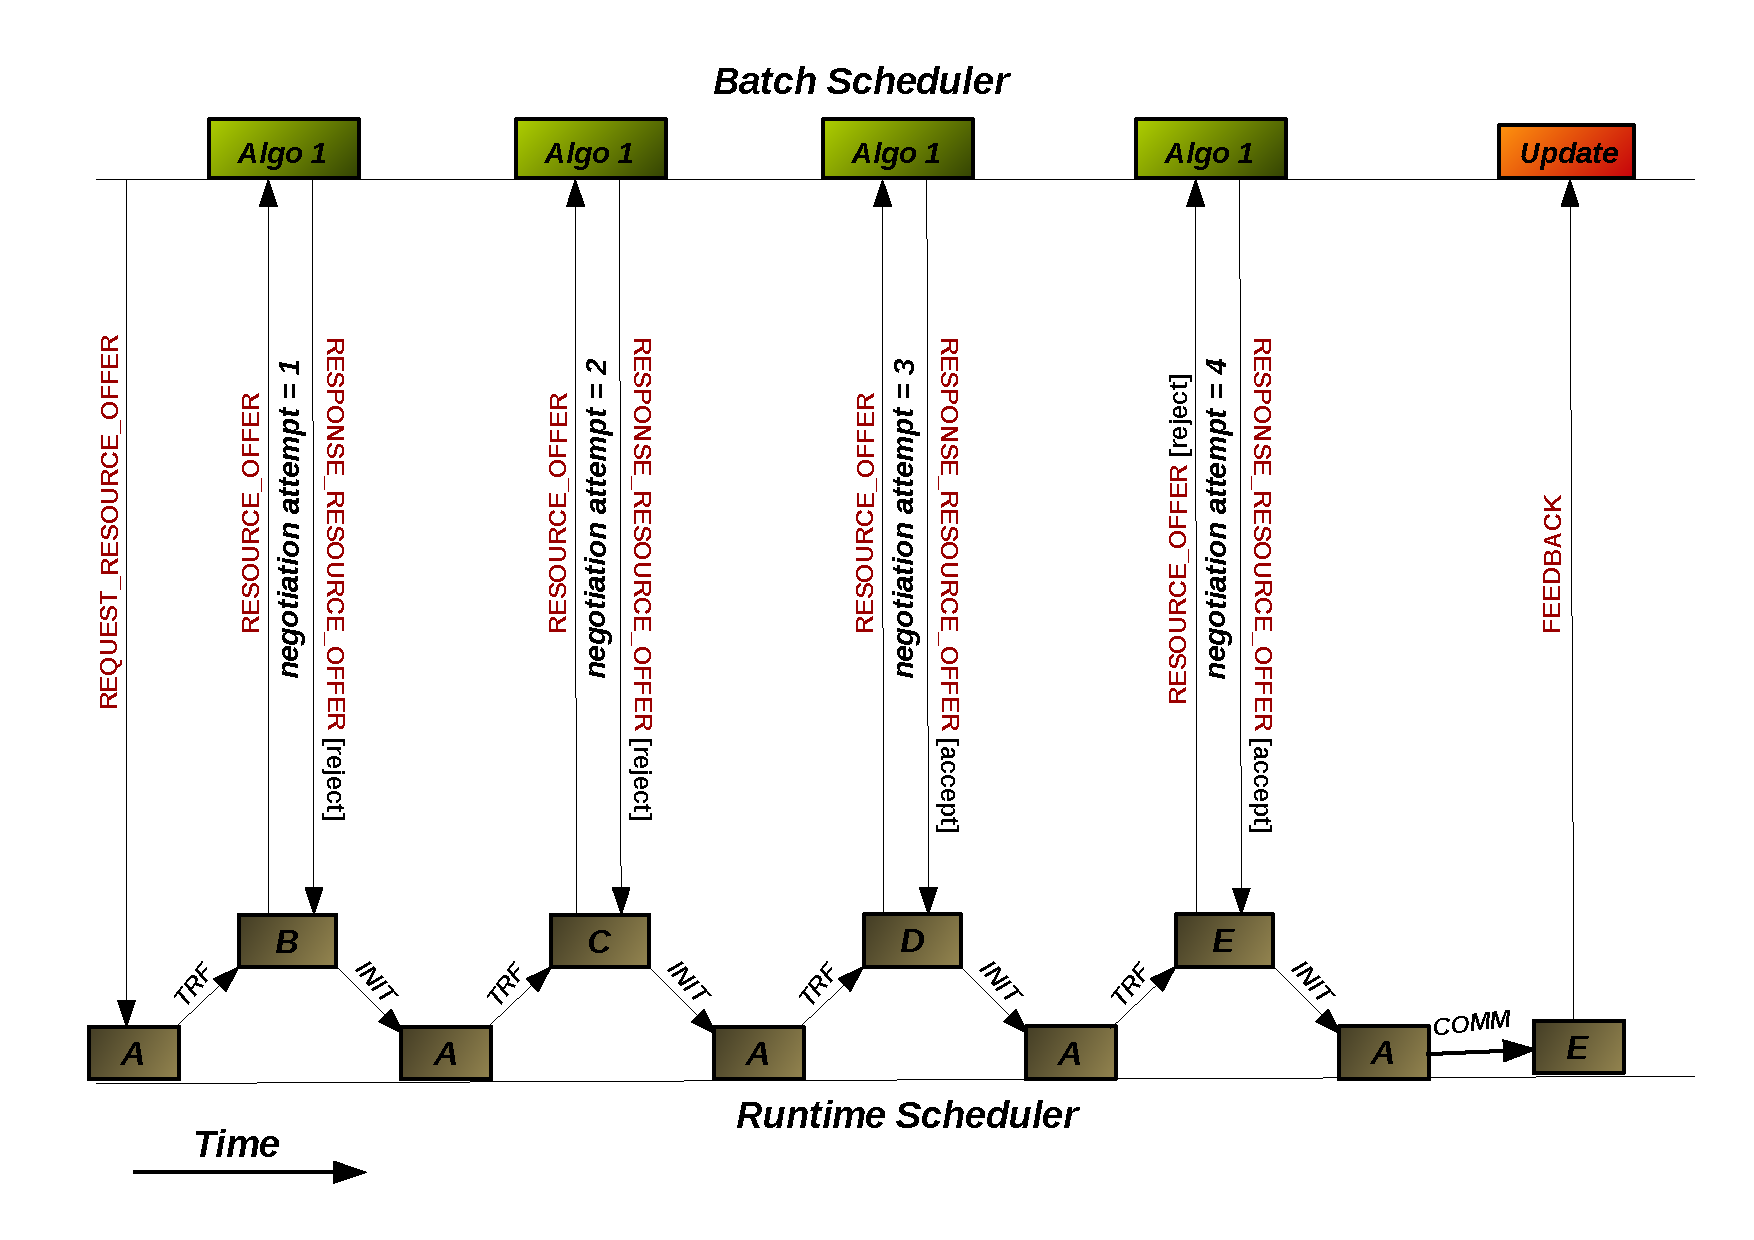
\includegraphics[width=1.2\textwidth, height=120mm]{./figures/negotiation.pdf}
\caption{Negotiation protocol}
\label{fig:2}
\end{figure}
